% Tabellen, Transaktionen, Endpunkte
\section{Technische Kontextabgrenzung}
% TODO Quelle Database per Service vs Shared Database
Bei der Modellierung der Datenbankschicht wurde das Database-per-Service Muster verwendet. Dieses Muster erlaubt eine sehr lose Bindung der Services und lässt die Datenbasis in der Verantwortung eines Services. Es ist möglich, ein Microservice-System zu implementieren, welches das Muster einer gemeinsamen Datenbank verwendet. Dies würde die Implementierung atomaren und konsistenten Transaktionen vereinfachen. Die Voraussetzungen für eine solche Implementierungen sind jedoch nicht immer gegeben, da an der LLT teilhabende Services unter Umständen nicht in der Verantwortung des Entwicklerteams liegen könnten, welches die LLT zu implementieren hat. Aus diesem Grund wird im Rahmen der für diese Implementierung vorzunehmende Implementierung jeder Service als getrennte Komponente aufgefasst, die als alleinige Instanz auf ihre eigenen Daten zugreift und zugreifen kann.

% TODO vereinfachte Darstellung der Schnittstellen im folgenden, ausführliche Beschreibung in Swaggerfile im Anhang

\subsection{ArticleService}
\paragraph*{Datenbankschicht}

Der ArticleService soll lediglich Daten aus der Datenbanksicht zurückliefern. Deshalb wird für diesen Service lediglich eine Tabelle benötigt. Die Tabelle \textit{article} enthält für jeden anzubietenden Artikel den zugehörigen Namen und Preis.

\begin{figure}[h!]
	\centering
	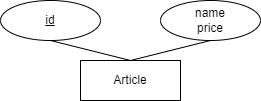
\includegraphics[scale=0.5]{figures/DatabaseER/ArticleServiceTables.png}
	\caption{ER-Diagramm ArticleService}
\end{figure}
\FloatBarrier

\paragraph*{Schnittstellen} \mbox{}\\
% TODO RESTful, Ressource
Die Produktdaten sollen von dem Frontend abgefragt und dargestellt werden. Dabei werden alle vorhandenen Produktdaten selektiert und zurückgegeben. 

Zusätzlich soll der Koordinator eine gezielte Abfrage durchführen können, welche den Preis eines Artikels für eine gegebene ProduktId liefert. Beide Schnittstellen sind RESTful, da jeder Artikel als Ressource angesehen wird. 

Da eine Bestellung mehrere unterschiedliche Artikel enthalten darf, wird zusätzlich eine Schnittstelle angeboten, die dem Aufrufer ermöglicht, mehrere Artikel per Id aufzulösen. Die angefragten ArtikelIds werden als Queryparameter übergeben.

\begin{center}
	\begin{tabular}[h]{|p{3.5cm}|p{3cm}|p{6cm}|}
		\hline
		Endpunkt & Http-Methode & Argumente \\ \hline
		/api/articles & GET & optionale Einschränkung der Ids per Queryparameter \\ \hline
		/api/articles/\{id\} & GET & ArticleId \\ \hline
	\end{tabular}
\end{center}
\FloatBarrier

\subsection{StockService}
\paragraph*{Datenbankschicht} \mbox{}\\

Der StockService verwaltet vier Tabellen. Die zentrale Tabelle ist \textit{articlestock} und stellt für jeden bekannten Artikel den auf Lager befindlichen Vorrat dar. Eine Reservierung für eine gegebene Vorgangsnummer wird in der Tabelle \textit{blockedarticles} durch alle Tupel, bei denen diese Nummer auftritt. Die Lieferungen werden in der Tabelle \textit{shipments} dargestellt. Auch hier gehört eine Vorgangsnummer zu den Spalten. Zusätzlich gibt es das Attribut \textit{hasarrived}, was Auskunft über den Status der Lieferung gibt. Die zu einer Lieferung gehörenden Artikel und deren Menge sind in der Tabelle \textit{shippedarticles} enthalten.

\begin{figure}[h!]
	\centering
	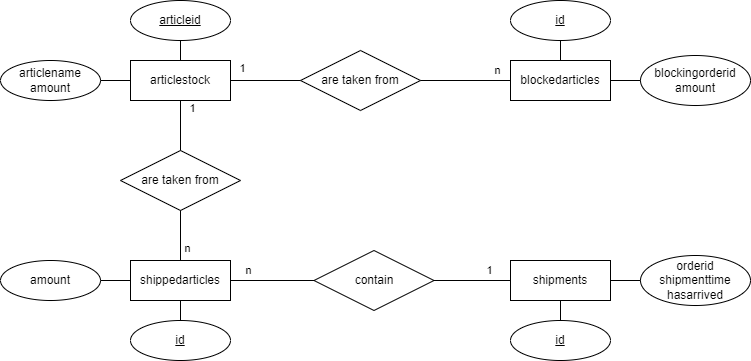
\includegraphics[scale=0.5]{figures/DatabaseER/StockServiceTables.png}
	\caption{ER-Diagramm StockService}
\end{figure}
\FloatBarrier

\paragraph*{Schnittstellen} \mbox{}\\

Der Endpunkt \textit{/api/blocked-articles} überträgt frei verfügbare Artikel aus der Tabelle \textit{articlestock} in die Tabelle \textit{blockedarticles}. Als Argumente werden die zu blockierenden Artikel-Ids und Artikel-Mengen sowie die Vorgangsnummer benötigt. Teil der lokalen Transaktion sind folgende Schritte:
\begin{enumerate}
	\item Reduzieren jedes Artikelvorrats in der Tabelle \textit{articlestock}
	\item Einfügen eines Elements in der Tabelle \textit{blockedarticles} für jede zu blockierende Artikel-Id
\end{enumerate}

Der Endpunkt \textit{/api/blocked-articles-compensation} stellt die Kompensierung für die Schnittstelle \textit{/api/blocked-articles} dar. Als Argument wird hier lediglich die Vorgangsnummer benötigt. Notwendige Schritte der auszuführenden lokalen Transaktion sind:
\begin{enumerate}
	\item Selektieren aller Elemente aus \textit{blocked-articles} mit der angefragten Vorgangsnummer
	\item Löschen dieser Elemente
	\item Erhöhen der Vorratsmengen in \textit{articlestock} für jede Artikelblockierung
\end{enumerate}

Der Endpunkt \textit{/api/start-shipment} erwartet die Vorgangsnummer als Argument. Die reservierten Artikel werden in eine Lieferung umgewandelt und versendet. Die Schritte der ablaufenden lokalen Transaktion sind:
\begin{enumerate}
	\item Initialisieren eines Elements in \textit{shipments} mit dem Status \textit{hasarrived=0}
	\item Selektieren und Löschen aller Elemente in \textit{blockedarticles}, die die OrderId enthalten
	\item Einfügen der Selektierungen in der Tabelle \textit{shippedarticles}
\end{enumerate}

Der Endpunkt \textit{/api/finish-shipment} wird ausschließlich vom Lieferanten verwendet und dient zur Bestätigung der Lieferung. Es wird der Status der entsprechenden ShipmentId in der Tabelle \textit{shipments} auf 1 gesetzt.

Der Endpunkt \textit{/api/shipments} liefert den Status der angeforderten ShipmentId. Der Koordinator hat mit dem Aufruf von \textit{/api/start-shipments} die Lieferung ausgelöst. Der Koordinator hat mit der Schnittstelle \textit{/api/shipments} die Möglichkeit, den Status der Lieferung solange abzufragen, bis der Lieferant per Aufruf von \textit{/api/finish-shipment} den Lieferabschluss bestätigt. Die Kombination von \textit{/api/start-shipment}, \textit{/api/finish-shipment} und \textit{/api/shipments} können als Polling-Implementierung eines asynchronen Request-Response Musters aufgefasst werden. 

Der letzte Endpunkt des StockServices ist \textit{/api/cancel-shipment} und bietet dem Koordinator die Möglichkeit, auf eine Stornierung zu reagieren. Bis die Lieferung abgegeben und bestätigt wurde, kann diese Schnittstelle verwendet werden, um die Lieferung abzubrechen. Als Argument wird die ShipmentId benötigt.

\begin{center}
	\begin{tabular}[h]{|p{6.5cm}|p{3cm}|p{5.1cm}|}
		\hline
		Endpunkt & Http-Methode & Argumente \\ \hline
		/api/blocked-articles & POST & ArticleId, Amount, OrderId\\ \hline
		/api/blocked-articles-compensation & POST & OrderId \\ \hline
		/api/start-shipment & POST & OrderId \\ \hline
		/api/finish-shipment & POST & ShipmentId \\ \hline
		/api/shipments & GET & ShipmentId \\ \hline
		/api/cancel-shipment & POST & ShipmentId \\ \hline
	\end{tabular}
\end{center}
\FloatBarrier

\subsection{BankingService}
\paragraph*{Datenbankschicht} \mbox{}\\
% TODO Tabellenbezeichnungen anpassen
Zur Verwaltung des BankingServices gehören drei Tabellen. Die Tabelle \textit{bankuser} enthält alle Nutzer, die Tabelle \textit{bankusercredit} ordnet jedem Nutzer einen Kontostand zu und die Tabelle \textit{bankusertransaction} stellt Veränderung des Kontostands der Tabelle \textit{bankcredit} in der Tabelle \textit{bankusertransaction} als Historie dar.

\begin{figure}[h!]
	\centering
	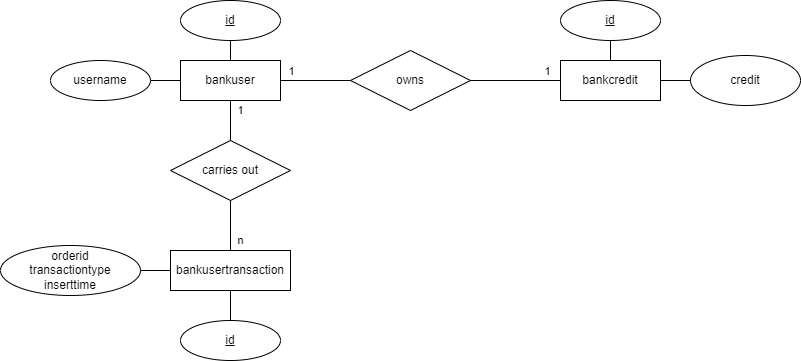
\includegraphics[scale=0.5]{figures/DatabaseER/BankingServiceTables.png}
	\caption{ER-Diagramm BankingService}
\end{figure}
\FloatBarrier

\paragraph*{Schnittstellen} \mbox{}\\
Der BankingService bietet jeweils eine Schnittstelle zum Erhöhen und zum Verringern des Kontostandes an. Dabei wird lediglich in der Tabelle \textit{bankcredit} das Credit-Attribut erhöht oder verringert. Die Spalte ist im Datenbankmanagementsystem mit einer Einschränkung versehen, die verhindert, dass der Wert der Spalte unter 0 fällt. 

Die Veränderung des Kontostandes ist der erste Schritt der lokalen Transaktion. Der zweite Schritt ist das Einfügen eines neuen Elementes in der Tabelle \textit{bankusertransaction}. In dieser Tabelle wird der Transaktionstyp festgehalten. 

\begin{center}
	\begin{tabular}[h]{|l|l|l|}
		\hline
		Endpunkt & Http-Methode & Argumente \\ \hline
		/api/add-money & POST & UserId, Amount, OrderId \\ \hline
		/api/add-money-compensation & POST & UserId, Amount, OrderId \\ \hline
		/api/remove-money & POST & UserId, Amount, OrderId \\ \hline
		/api/remove-money-compensation & POST & UserId, Amount, OrderId \\ \hline 
	\end{tabular}
\end{center}
\FloatBarrier